\section{Implementation}
This project was developed over 8 sprints of between 7-10 days each with the first one started on the 26th of December, 2022 and the last one stared on March 19, 2023. What follows is a detailed summary of the work done during those sprints divided into three subsections:
\begin{itemize}
    \item Plan - Highlights what user stories were chosen to be implemented during the sprint and how long that sprint was.
    \item Implementation - How the features were implemented, any design decisions and any issues
    \item Summary - Have all user stories been completed? What went wrong? Anything learned and moved to next sprint
\end{itemize}

\subsection{Sprint 1 - Start 26th December}

\subsubsection{Plan}
This was the first sprint undertaken for the project and so the focus was to test everything out and ensure that the process was right for the student. The initial MVP feature set was chosen for development and two user stories were planned for. Those being user stories 3 and 11 with a total workload estimate of 6 over a 7 day sprint.
The main goal for this sprint was to create a labelled scatterplot graph with some pre-set test data.

\subsubsection{Implementation}
Prototype 2 was chosen to be extended into the application being developed. It was copied into the development branch and work started on implementing the user stories mentioned. A 3D Cube with axis lines was created as the chart and an origin position was set from which data points would be rendered. This was not as difficult as expected as the model matrix used could be copied and modified by each data point to ensure that they were always at a correct position relative to the cube and axis lines.

The next step was to label the axis lines (also relative to the chart using it's model matrix). This caused some difficulty as test labels would not align properly even if they were supposed to based on their coordinates. This was particularly troublesome with perspective lines that had a considerable z change in position. This was found to be a result of inaccurate placement by the browser (browsers favors flexibility over screen sizes instead of rigid pixel-perfect placement) and not fully correct world to screen coordinate calculation. Instead, it was decided that text should be rendered within the WebGL scene to ensure accuracy- To that end, a bitmap font technique was adopted.

\begin{figure}[h]
    \centering
    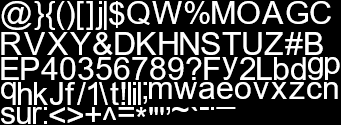
\includegraphics[width=0.5\columnwidth]{author-files/figures/glyphset.png}
    \caption{Arial font bitmap glyph image}
    \label{fig:arial}
\end{figure}

This is where a texture atlas with pre-rendered glyphs is downloaded and used to apply individual glyphs to flat surfaces (usually two triangles of geometry). This technique was mainly adopted due to it's simpler implementation and higher performance over the main alternative of using a geometric approach for rendering text (Where geometry is used to shape each glyph, which uses much more triangles). This alternative is highly inefficient as geometry is computationally expensive to render. Although it should be noted that bitmap font's do also carry their own limitations, mainly it is difficult to have large character sets as each character set would need to be saved into an image and downloaded, which if changing font sizes is required further requires that different sized copies of the character sets are available to avoid blurriness and pixelation at large sizes.
For this project though, those were considered to be tolerable limitations. Blurriness could be avoided by keeping glyphs the same size and the limited glyph set wouldn't matter as much with only one supported application language.
With bitmap fonts decided upon, the student started work on adapting the application to support rendering text in this way. This required a couple of key changes and additions within the renderer part of the application:
\begin{itemize}
    \item It should be possible to apply textures to models- This was done by adapting the Model class to store and apply texture data on render
    \item Textures had to rendered and stored- This was done by expanding the Loader class to allow .png images to be loaded
    \item There had to be some way to abstract which letter was rendered, manually slicing the bitmap texture to get each glyph would quickly become too tedious and time consuming for anything beyond a few glyphs- A State-Machine based Font Class was created that generated font texture data for an input letter that could be fed into a Model Object.
\end{itemize}

Have some class diagram here

\subsubsection{Summary}
The new technique for rendering text ended up fixing the accuracy issues caused by the previous label system and all user stories managed to be completed as expected and the application was pushed to production on january 1st, 2023. This was a slow start but the student expected that more user stories would be able to be tackled as they progressed with the project.

\subsection{Sprint 2 - Start 4th January}
\subsubsection{Plan}
This was the second sprint and the plan was to start adding user controls to allow a user to modify what was being rendered. This included not only the ability to upload custom data but also rotate the resultant graph. The MVP feature set was again the developed feature set from which 4 user stories were selected, with a total work load estimate of 16 over a longer 11 day sprint. This was originally a 7 day sprint but an extension was deemed necessary to have an atomic conclusion to the sprint. In total, 16 Units of work were completed for an average of 8 per week.

\subsubsection{Implementation}
Loader was once again expanded to handle .csv loading which was done using jquery-csv, which sped up development considerably and covered a lot of edge cases in possible file uploads. For user controls, the use of modern UI frameworks was considered but at this moment in time- there wasn't much UI requirement for the application. Instead, as per PXP, the student focused on hitting user stories as fast as possible. Thus, an observer like structure was implemented using Event listeners connected to overlaid HTML Elements on the page (In a similar way to how the old label system worked, See Sprint 1) which ran functions that modified the state of the application. With this design, 6 buttons were made to rotate each axis of the chart individually. Another button was added to upload a file that was handed to Loader.

\subsubsection{Summary}
This was almost a double sprint. This was mainly due to lower work hours done by the student during the winter vacation. Nevertheless, All user stories were completed and the application was pushed to production on January 29th. This delay was due to the previously mentioned lower hours and semester start travel. At this point, a technically functional plotter was created, though still very limited in functionality.